\chapter{Two level graph matching} \label{chapter:2levelGM}
In this chapter we describe our novel approach for graph matching. Our aim was not to develop a new matching algorithm, but to propose a framework, which would help to solve problems, where direct application of an existing matching algorithm is impossible due to memory requirements or performance time. This is often the case when a graph matching problem is formulated using a similarity matrix between graphs. Our main idea is based on the  \emph{divide and conquer} technique~\cite{Cormen}, which is well known from its application to array sorting algorithms. According to this general paradigm, a given graph matching problem, which is too difficult to be solved directly, is subdivided into smaller subproblems, those can be solved without great effort. A resulting solution is then combined from a local solutions of single subproblems. Important properties of such approach are its runtime improvement and not significant drop in accuracy. Desirable is off course also an improvement in the accuracy.

There are already several algorithms, which share the similar ideas. Those, which are most closed to our approach were described in previous chapter under algorithms based on clustering techniques. Below we review them shortly again to point out, that none of them completely repeat our framework.

This chapter is organized we follows. First of all, we formulate considered graph matching problem and show some issues of this formulation. In the second part, we describe our two level graph matching framework, which should help to cope with formulated problems. The performance results and comparison with other algorithms are summarized in the next chapter. 
% ---------------------------------       Problem Statement      -------------------------------------
\section{Problem statement} \label{sec:prob_stat}
Consider two attributed graphs $G^I = (V^I, E^I, D^I)$ and $G^J = (V^J, E^J, D^J)$, where $V$, $E$, $D$ denote set of nodes, set of edges and set of node attributes respectively. We assume the situation, where those graphs are undirected and do not have multiple edges between nodes. Let the size of the first graph be $n_1$ and the second $n_2$. Without loss of generality, we assume that $n_1\le n_2$. Attributes of the graphs are $k-$dimensional real vectors: $D^I,D^J\in\mathbb{R}^k$.

We define a problem of matching two graphs $G^I$, $G^J$ as a quadratic assignment problem (same formulation as~\eqref{eq:gQAP1}-\eqref{eq:gQAP4}). 
\begin{alignat}{2}
    &     && \argmax_x{x^TSx}                           \label{eq:gQAP1_2}\\
    & \text{s.t. } &&  x\in \{0,1\}^{n_1n_2}            \label{eq:gQAP2_2}\\
    &             &&  \sum_{i=1\dots n_1} x_{ij}\le 1   \label{eq:gQAP3_2}\\
    &             &&  \sum_{j=1\dots n_2} x_{ij}\le 1   \label{eq:gQAP4_2}
\end{alignat}
We denote a pair of nodes $(v_i,v_j)$, where $v_i\in V^I$ and $v_j\in V^J$, as a correspondence between the sets $V^I$ and $V^J$. Let $M$ be a set of all possible correspondences between the nodes of the graphs $G^I,G^J$. Obviously, $M$ consists of $n_1n_2$ node pairs.  Then the vector $x\in \{0,1\}^{n_1n_2}$ is an indicator vector of a subset $m=\{(v_i,v_j)|v_i\in V^I,v_j\in V^J\}$ of the $M$. That means, that element $x_k$ of this vector is equal $1$ if and only if the corresponding k-th node pair $(v_i,v_j)$ is selected into subset $m$. The constraints~\eqref{eq:gQAP3_2},~\eqref{eq:gQAP4_2} ensure, that each node of the graph $G^I$ is matched to exactly one node of the second graph $G^J$.

The matrix $S\in\mathbb{R}^{n_1n_2\times n_1n_2}$ in~\eqref{eq:gQAP1_2} encloses the precomputed information about similarity of two graphs. Rows (columns) of this matrix correspond to the elements in the set $M$ of all possible node correspondences. Its diagonal element $S_{kk}$ contains similarity measurement of the node pair $(v_i,v_j)_k\in M$. On the other side, the non-diagonal elements of $S_{kl}$ measure similarity of edges between two pairs of matched nodes. Our aim is to find a subset of maximal $n_1$ correspondences between the nodes of the graphs $G^I,G^J$, which maximizes the similarity value between those graphs.

As we saw in the previous chapter, the selected formulation of a graph matching problem is widely used as the most general one. However, the size of the affinity matrix $S$ can cause problems due to required memory demand. For example, a dense affinity matrix between two graphs with $200$ nodes each needs approximately 12Gb memory (double precision). There are several possible ways to reduce the memory complexity of the formulated graph matching problem. Here we mention tree possible approaches.

The first one is to reduce a set of candidate correspondences by selecting a subset $M^\prime\subset M$. This can be done, for example, by restricting a number of candidate matches for a node $v_i\in V^I$ to some number smaller than $n_2$. This method is often used, as it not only solves memory issue of the problem formulation~\eqref{eq:gQAP1_2}-\eqref{eq:gQAP4_2}, but also reduces the algorithmic complexity of many algorithms, which highly depend on the number of possible matches~(e.g.~\cite{Cho2014_Haystack,Cho2010_RRWM,Cho2012_ProgressiveGM, Leordeanu2005_SM}).

The second possibility, is to make the matrix $S$ sparser by excluding comparison of some nodes or edges from consideration. In case of a big graphs this can however lead to a high loss of initially provided information and results dramatically on the quality of a resulting matching. 

The third possibility is to replace an initial problem of graph matching by a set of smaller subproblems by partitioning given graphs into subgraphs and matching those subgraphs. For the matrix $S$ it means, that it is divided into blocks, where each block represent a similarity matrix between two subgraphs. Thereby the similarities of edges, whose nodes belong after problem splitting to different subgraphs, will be ignored. On the one hand, this approach solves the memory problem by replacing the initial matrix $S$ with a set of smaller affinity matrices. On the other hand, it does not reduces the algorithmic complexity of the initial problem, because the subgraphs of two graphs should be matched in all possible combinations between each other. Otherwise, further information will be lost. Despite the mentioned drawbacks, single subgraph matching problems can be eventually parallelized, what still makes the approach attractive for application on big graphs.

In the framework for graph matching, that we describe in the details below, we use the third of described techniques. We divide a given initial graphs into subgraphs and iteratively search first for correspondences between the subgraphs and then for node correspondences between matched subgraphs. For subgraph matching we use some existing matching algorithm. A graph partitioning is performed only at the initialization step, but after each iteration subgraphs have a change to exchange nodes on their border.

To our best knowledge the described method was not published before. Especially, we haven not seen an iterative algorithm based on graph clustering so far, which would update initial partitions. At the same time there is a certain overlap in ideas between our and existing works. The algorithm proposed by Lyzinski et al.~\cite{Lyzinski2015} uses graph partitioning to parallelize a semi-supervised graph matching problem, where some correspondences between graphs nodes are provided. The graph matching problem is formulated as the minimization problem~\eqref{eq:QAP1}, that does not use an affinity matrix $S$. The given matches between graph nodes are used to cluster two graphs jointly and to find a correspondences between subgraphs. As a consequence, subgraphs of given graphs are similar enough to ensure the matching quality. However the proposed clustering method cannot be used for a unsupervised matching.

The similar idea to our to use graph partition for graph matching in unsupervised case was used by Carcassoni and Hancock~\cite{Hancock_ModalClusters}, Qui and Handcock~\cite{Hancock_GM_SpectralPart} and recently by Nie et al.~\cite{CliqueGraph_CVPR2015}. From them only the third algorithm consider the same maximization problem as we. The two other algorithms formulate graph matching problem in terms of relaxation labeling. Also the definition of the graph clusters differs between the algorithms. Qui and Hancock, as well as Nie et al., consider clusters, that are built by a direct neighborhoods of nodes. The resulting partition can be overlapping~\cite{CliqueGraph_CVPR2015} or not~\cite{Hancock_GM_SpectralPart}. Our algorithm and the one in~\cite{Hancock_ModalClusters} consider more general case, where a graph partition is given by a disjoint set of graph subgraphs.
Finally, similar to our approach Qui and Handcock~\cite{Hancock_GM_SpectralPart} use the extracted graph partitioning to create a new graph, whose nodes represent clusters of initial graphs. They call this process graph simplification. However their approach quite differs from our, because of special definition of clusters, another problem formulation and different approach for solving single matching problems, as we mentioned above.

In the remainder of this paper we describe in details our graph matching approach.

% ---------------------------------------    Approach       ------------------------------------------
\section{Algorithm}
We consider at the beginning only one graph $G^I=(V^I,E^I,D^I)$ of the size $n_1$. Assume, that we know a partition of the node set $V^I$ of this graph into $m_1$ non-overlapping clusters based on some rule: $V^I=\cup_{k=1}^{m_1}V^I_k$, where $V^I_{k_1}\cap V^I_{k_2}=\emptyset$ for $k_1\not=k_2$. Based on this partition the initial graph $G^I$ is subdivided into a set of node induced subgraphs $\{G[V^k]\}_{k=1}^{m_1}$. Note, that it holds $G[V^1]\cup\dots\cup G[V^{m_1}]\subset G^I$, because edges between different subgraphs are note presented in the left union.
Further, we define a mapping $U$ between the set of graph nodes $V^I$ and another set of nodes $V^{Ia}=\{a^I_k\}_{k=1}^{m_1}$, which represent each subgraph  $G[V^I_k]$ with a single node $a^I_k$. This mapping can be expressed as an matrix $U^{Ia}\in\{0,1\}^{n_1\times m_1}$ with elements 
\begin{equation*}
U^{Ia}_{ik} = \begin{cases} 1, & \mbox{if node } v_i\in V^I_k,    \\
0, & \mbox{otherwise}.\end{cases}
\end{equation*}
The new set $V^{Ia}$ defines a node set of a new graph built on top of the other. A pair of new nodes $a^I_{k_1},a^I_{k_2}\in V^{Ia}$ is connected with an edge, if there is at least one edge in the initial graph $G^I$ between the corresponding clusters $V^I_{k_1}$ and $V^I_{k_2}$. The set $V^{Ia}$ together with the set of edges between its elements and correspondence matrix $U^{Ia}$ build a new graph $A^I=(V^{Ia},E^{Ia},U^{Ia})$. We will call the graph $A^I$ an \emph{anchor graph} of the graph $G^I$ and its nodes \emph{anchor nodes} or just \emph{anchors}. The graph $G^I$ together with its anchor graphs $A^I$ build a two level system: the graph $G^I$ is located on the lower (finer) level and the graph $A^I$ on the higher (coarser) level (see Fig. \ref{fig:2levels}).

\begin{figure} [h!]
	\centering
	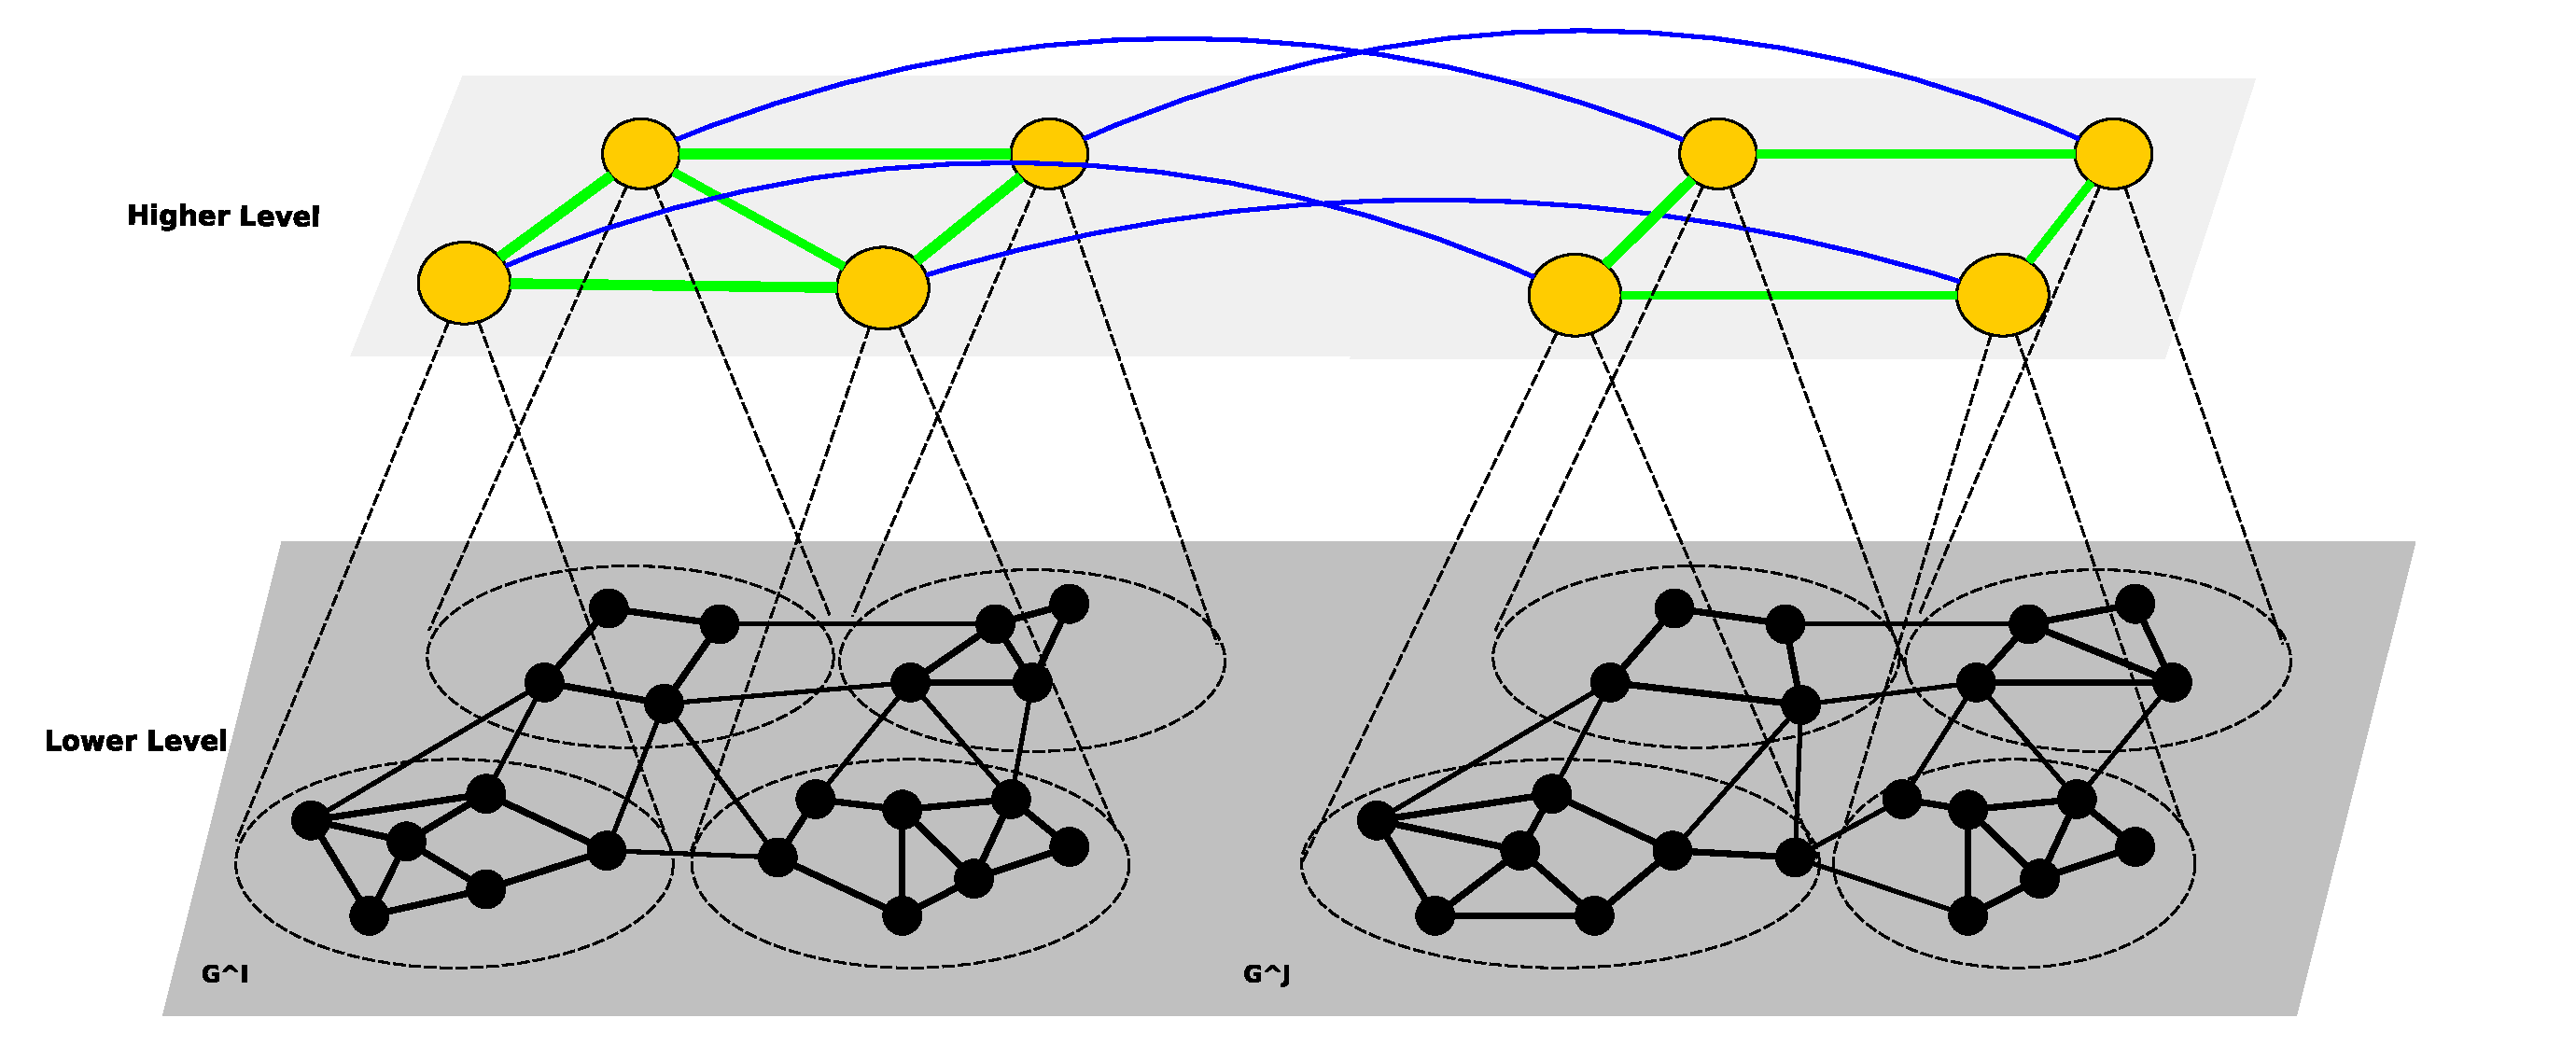
\includegraphics[scale=0.35]{chapter2/fig/twolevels2.pdf}
	\caption{Two level framework for graph matching} \label{fig:2levels}
\end{figure}

We return now back to the case of two graphs $G^I=(V^I,E^I,D^I)$ and $G^J=(V^J,E^J,D^J)$, which we want to match. 
For each of them we build an anchor graph $A^I=(V^{Ia},E^{Ia})$ and $A^J=(V^{Ja},E^{Ja})$ respectively.
Now instead of matching graphs $G^I$ and $G^J$ directly on the lower level, we may want to match first the corresponding anchor graphs. Matches between anchor nodes give us correspondences between underlying subgraphs. After that, we can perform graph matching for each pair of subgraphs completely independently. A union of local solutions from single subgraph matching problems gives us a solution of initial problem. 

Why this approach can be better than direct one? As we seen from the previous section the complexity of the considering graph matching problem depends highly on the size if initial graphs. Constructed anchor graphs are however several time smaller than initial graphs, which means, the matching algorithm on the anchor level can be performed much faster then on the lower level. The same holds for matching between the subgraphs.
%If $C(n)$ is complexity of a graph matching algorithm with $n$ possible correspondences.
Obviously, the accuracy of such two level matching approach depends heavily on the partition of the initial graphs into subgraphs and on the matching quality of the anchor graphs. To make the described two level approach more robust again graph partitioning we suggest to perform described steps iteratively till convergence of the objective function~\eqref{eq:gQAP1_2}. On each iteration we want to use an obtained matching between two graphs to correct graph partitioning. The algorithm is summarized below in Alg.\ref{alg:2levelGM}.

\begin{algorithm}[h]
	\KwIn{ initial graphs $G^I$, $G^J$\\
		   \hspace{45pt}maximal number of iterations $N$\\
		   \hspace{45pt}convergence parameters $R$ and $\epsilon$}
	\KwOut{set $m$ of correspondences between the nodes $V(G^I)$ and $V(G^J)$}
	construct anchor graph $A^I$ of the graph $G^I$ \label{alg:2levelGM_clustering1}\\
	construct anchor graph $A^J$ of the graph $G^J$ \label{alg:2levelGM_clustering2}\\
	i=0, $score_i$=0\\
	\While{$r<R$  \textbf{AND} $i\le N$}
	{ $i=i+1$ \\
	  \If{$i\ge 2$}
	  {update subgraphs $G[V^I_k],G[V^J_p],k=1\dots,m_1,\ p=1\dots,m_2$ \label{alg:2levelGM_update}}
	  match anchor graphs $A^I$,$A^J$ \label{alg:2levelGM_GM1} \\
	  $m_i=\emptyset$\\
	  \ForEach{pair of matched anchors $(a_k,a_p),a_k\in V(A^I), a_p\in V(A^J)$}
	  {match subgraphs $G[V^I_k]$,$G[V^J_p]$ \label{alg:2levelGM_GM2}\\
	   $m_i=m_i\cup\{m^k_i\}$\hspace{55pt}\tcc{$m^k_i$ set of local correspondences}
	  }
	  $score_i=x^TSx$ \hspace{5pt}\tcc{$x$ the indicator vector of the subset $m\subseteq M$}
	  \If{$|score_i-score_{i-1}|<\epsilon$}
	  {$r=r+1$}
	  \Else{$r=0$}
	}
	\Return $m_i$
	\caption{twoLevelGM($G^I$, $G^J$, $N$, $R$, $\epsilon$)} \label{alg:2levelGM}
\end{algorithm}

In the following we describe in details the single steps of our approach: %initial graph construction,
graph partitioning~(lines~\ref{alg:2levelGM_clustering1},\ref{alg:2levelGM_clustering2}), graph matching algorithm on both levels~(lines~\ref{alg:2levelGM_GM1},\ref{alg:2levelGM_GM2}), as well as update rules of graph partitions from a previous level~(line~\ref{alg:2levelGM_update}).
\FloatBarrier
% ---------------------------------------        HLG Construction
\subsection{Anchor Graph Construction}
A problem of anchor graph construction given an initial graph $G^I=(V^I,E^I,D^I)$ turns straight forward into problem of partitioning the graph $G^I$. During our work on this thesis we tried out different strategies for clustering nodes of a given graph. Here we present those, which were more suitable for our matching framework, however generally an arbitrary algorithm for graph partitioning can be used.

Here and further we assume that the nodes of the given fine graph $G^I$ are located on a plane. That means, for each node we have additionally to its attribute an associated pair of coordinates and therefor can define the length of an edge as a $l_2-$distance between its endpoints.
\subsubsection{Using grid}	
The first algorithm we describe is the most simple one. It uses a grid with fixed number of rows $r$, columns $c$ and a cell width $w$. The grid is placed over the graph $G^I$. Nodes, that are captured by a same grid cell belong to one cluster. Obviously, the number of clusters is equal to $r\times c$. We place anchor nodes in the middle of the grid cells. Two anchors are connected by an edge, if the cells they belong to have a common edge.
\subsubsection{Algorithms based on node merge}
The next considered approach creates an anchor graph $A^I$ with a predefined number $m_1$ of anchors. For that we adopted a coarsening phase from multi-level graph partition algorithms \cite{Chevalier09_GP, Safro2012_GC, Karypis95_GP, Hendrickson1995}.
Such algorithms have generally three phases: 
\begin{enumerate}
	\item graph coarsening phase, where one creates a hierarchy of graphs by successive merging of nodes in graph on previous stage starting with initial graph;
	\item graph partition stage, where the partition problem is solved exact on the coarsest level;
	\item refinement phase, where solution of the coarsest level is interpolated through all levels of the hierarchy until the initial graph.
\end{enumerate}
There are several types of graph coarsening algorithms. In our work we used so-called strict aggregation scheme (SAG)~\cite{Chevalier09_GP}, which groups nodes of $G^I$ in disjoint subsets based on the strength of the edges between them. We implemented two SAG based algorithms: Heavy Edge Matching (HEM) and Light Edge Matching (LEM)~\cite{Chevalier09_GP}. Both algorithms visit nodes of the graph $G^I$ in random order and construct an independent set of edges $M$ of the graph. The edge selection is based on the edge weights. The HEM picks and adds into $M$ the strongest edge adjacent to a current node $v$, that does not belong to the set of end nodes of edges in $M$.~(see Alg.~\ref{alg:HEM}). As opposed to this, the LEM selects the weakest edge adjacent to a current node. The edges in $M$ will be contracted, i.e. their endpoints will be replaced with a new node, that lies in the middle of a contracted edge and is connected to all neighbors of its endpoints.

{\LinesNumberedHidden
\begin{algorithm}[h]
	i = 0, $M=\emptyset$ \\
	\While{$|V(G^I)|>m_1$  \textbf{AND} $i\le N$}
	{ select a random node $v\in V(G^I)\setminus V(M)$ \\
	  \If{$\exists v^\prime=\argmax_{u\in V(G^I)\setminus V(M)} w(v,u)$}
	  {$M=M\cup{e_{vv^\prime}}$}
	  \Else{$i=i+1$}
	}
	\Return $G^I$
	\caption{HEM($G^I$, $m_1$, $N$)} \label{alg:HEM}
\end{algorithm} }

In out case, graph $G^I$ is not initially weighted. To use the described coarsening methods we need to define a strength of graph edges. In case of LEM-Algotihm we set the length of an edge as its strength: $w_{vv^\prime}=\|v-v^\prime\|_{2}$. If we use HEM-Algorithm the strength of an edge is equal to $w_{ii^\prime} = exp(-\frac{\|v-v^\prime\|_{2}}{\sigma^2_{s}})$ with a constant $\sigma^2_{s}$.

It is clear, that one iteration of HEM or LEM reduces the number of nodes in $G$ at most by $\lfloor\frac{n}{2} \rfloor$ nodes. To get an coarse graph with $m_1$ nodes the coarsening algorithm should be repeated several times.

\subsection{Anchor graph matching}
In the previous section we have described, how to construct anchor graphs $A^I=(V^{Ia},E^{Ia}, U^{Ia})$ and $A^J=(V^{Ja},E^{Ja},U^{Ja})$ of given graphs $G^I = (V^I, E^I, D^I)$ and $G^J=(V^J, E^J, D^J)$ respectively. Now, we focus our attention on the problem of matching two anchor graphs with. For that, according to our problem formulation~\eqref{eq:gQAP1_2}-\eqref{eq:gQAP4_2}, we need to define a similarity matrix $S^A\in\mathbb{R}^{m_1m_2\times m_1m_2}$ between the graphs $A^I$ and $A^J$, where $m_1=|V^{Ia}|$ and $m_2=|V^{Ja}|$. This matrix contains two types of similarities: edge similarities (non-diagonal elements) and nodes similarities (diagonal elements).

Consider two edges a pair of anchors  $a_k$, $a_k^\prime\in V^{Ia}$. We define the length of the edge $e_{kk^{\prime}}$ between those anchors as a mean of distances between nodes in the corresponding subgraphs $G[V^I_k]$ and $G[V^I_{k^\prime}]$. With other words:
\begin{equation} L_{kk^\prime} = \median_{\substack{v_i\in G[V^I_k]\\ v_{i^\prime}\in G[V^I_{k^\prime}]} }\|v_i-v_{i^\prime}\|_{2}, \end{equation}
where $\|v_i-v_{i^\prime}\|_{2}$ is the euclidean distance between the nodes $v_i\in G[V^I_k]$ and $v_{i^\prime}\in G[V^I_{k^\prime}]$.
Using this definition we calculate the similarity $s^A_E(e_{kk^\prime}, e_{pp^\prime})$ between edges $e_{kk^\prime}\in E^{Ia}$ and $e_{pp^\prime}\in E^{Ja}$ based on their length as it was done in the Eq.~\eqref{eq:edge_sim1}:
\begin{equation*}
s^A_E(e_{kk^\prime}, e_{pp^\prime}) = exp(-\frac{(L_{kk^\prime} - L_{pp^\prime})^2}{\sigma^2_{s}}).
\label{eq:s_e_A}
\end{equation*}

As we already discussed in the previous chapter, the comparison of graph nodes for determining node similarity is often based on the comparison of node attributes. However, our anchor graphs $A^{Ia}$, $A^{Ja}$ do not have direct attributes in contrast to the initial graphs $G^I$, $G^J$. Further we describe two ideas, which we suggest to calculate anchor similarities.

The first idea would be to assign some attributes to the anchors and proceed further in the same way, as for initial graphs. Definition of those attributes in the same way, as for nodes of original graphs, meaning taking into account only the anchor graphs and not considering underlying initial graphs, will probably not give us good results. The reason for this is, that two anchors with complete different subgraphs can get similar attributes and therefor are likely to be selected by a matching algorithm. If it happens, than the matching of the underlying subgraphs will have very low quality. This will have in turn an impact on the quality of the total matching of initial graphs. Consequently anchor attributes should incorporate the information about underlying subgraphs of original graphs.
Consider an anchor $a_k\in V^{Ia}$ and its underlying subgraph $G[V^I_k]=(V^I_k,E^I_k,D^I_k)$. We suggest two classes of attributes of the anchor $a_k$. 
\begin{itemize}
\item The first one uses a node attributes $D^I_k$ of the underlying subgraph $G[V^I_k]$. For this purpose we adopted \emph{bag of features model}~\cite{BoF_Leung2001}. We build once a common dictionary of all provided attributes in the both fine graphs by performing \emph{k-means clustering} of $D^I\cup D^J$ into $C$ clusters. Center of the clusters represent "codewords". Each attribute of a node in $V^I_k$ is afterwards mapped into the closest codeword. In this way, the anchor attribute $d_1(a_k)\in\mathbb{R}^C$ is defined as normalized histogram of "codewords" in corresponding subgraphs.

\item The second class of descriptors should capture the geometrical structure of underlying subgraph. We define $d_2(a_k)\in\mathbb{R}^{|V^I_k|\times b}$ as a set of $|V^I_k|$ histograms $\{d_2(a_k,v)\}$ with $b$ bins. Each histogram $d_2(a_k,v)$ represents a distribution of the length of the subgraph edges inside a small circle region around a node $v\in V^I_k$. 
\end{itemize}
The similarity value between two anchors can now be determined based on the first or second type of anchor descriptors. To calculate a distance between histograms we use $\chi^2$ statistic test \cite{Weken2004_ChiSqTest}:
\begin{equation}
s^A_1(a_k, a_p) = \sum_{b_i\in B}\frac{(d_1(a_k,b_i)-d_1(a_p,b_i))^2}{(d_1(a_k,b_i)+d_1(a_p,b_i)},
\end{equation}
\begin{equation}
s^A_2(a_k, a_p) = \frac{1}{|V^I_k|}\frac{1}{|V^J_p|}\sum_{v\in V^I_k}\sum_{u\in V^J_p} \big(\sum_{b_i\in B}\frac{(d_2(a_k,v,b_i)-d_2(a_p,u,b_i))^2}{(d_2(a_k,v,b_i)+d_2(a_p,u,b_i))}\big),
\end{equation}
where $a_k\in A^I, a_p\in A^J$ and notation $d_1(a_k,b_i)$ and $d_2(a_k,v,b_i)$ denote a value in the $b_i$-th bin of the corresponding histogram. 
Both similarities based on the anchor descriptors can be used separately or set together as a linear combination into one similarity function.

The second idea to determine similarity $s^A(a_k, a_p)$ between two anchors could be to perform graph matching of the underlying subgraphs $G[V^I_k]$, $G[V^J_p]$ and take its score as a similarity measure. This idea has a great drawback of high computational complexity, because we need to perform in summary $m_1m_2$ local matches. However, in this case the objective function of the global matching problem and the one on the anchor level are closer related. Among other, the both should have the same trend during the optimization process.~\ToDo{Check}
% --------------------------        LLG Construction          ---------------------------------------
\subsection{Subgraph matching}
Given two corresponding subgraphs $G^I_{k}=(V^I_{k},E^I_{k},D^I_{k})$ and $G^J_{p}=(V^J_{p},E^J_{p},D^J_{p})$. We use cosine similarity of the node attributes to calculate node similarity between $V^I_{k}$ and $V^J_{p}$. For the pairwise edge similarity we used the same formula as in case of anchor matching (see Eq.\eqref{eq:edge_sim1}), i.e.\ 
\begin{equation*}
s_E(e_{ii^\prime}, e_{jj^\prime}) = exp(-\frac{(l_{ii^\prime} - l_{jj^\prime})^2}{\sigma^2_{s}})
\end{equation*}
where $l_{ii^\prime}$, $l_{jj^\prime} $ are the lengths of edges $e_{ii^\prime}\in E^I$ and $e_{jj^\prime}\in E^J$ respectively.
%In our work we concentrate ourself on the task of finding feature correspondences between two images. Features are collected using such popular feature detectors as SIFT~\cite{Lowe2004}, MSER~\cite{MSER}. Extracted features from two images define the sets of nodes $V^I$, $V^J$ of the graphs $G^I$, $G^J$ respectively. As node attributes $D^I$, $D^J$ we used SIFT descriptors~\cite{Lowe2004} with fixed orientation and scale. 
%The nodes of the graphs are connected vie edges with their $k$ nearest neighbors.

% -------------------------        Matching algorithm              -------------------------
\subsection{Graph matching algorithm}
Generally, we are not restricted to use one specific algorithm for subgraph and anchor graph. We selected \emph{Reweighted Random Walks Method} (\textbf{RRWM})~\cite{Cho2010_RRWM}, as it shows high matching accuracy, according to result in the original paper, and is fast. It also showed good results in finding common subgraphs of two graphs in presence of outliers. At the end of this chapter we give for completeness an overview of the method.

% -------------------------        Level connection              -------------------------
\subsection{Connection between two levels}
Assume, we solved the GMP on the higher level. That means, we know pairs of correspondences between the anchor nodes: $m^a = \{(a_k, a_p)\}, a_i\in V^{Ia}, a_p\in V^{Ja}$. Since each anchor represents a subgraph of the initial graph, $m^a$ defines at the same time the correspondences between the subgraphs of the initial graphs $G^I$ and $G^J$. Solution of the $GMP$ for each pair of the subgraphs gives us the desirable correspondences between the nodes of the original graphs ($m = \{(v_i, v_j)\}, v_i\in V^{I}, v_j\in V^{J}$).

As we already mentioned above, the quality of the resulting solution $m$ depends in our framework not only on the quality of the graph matching algorithm, but also on the graph partitioning algorithm. The Fig.~\ref{fig:badpartition} shows, that by the fixed partition the matching results will be very pure for all possible matches of the anchors.

\begin{figure}
	\centering
	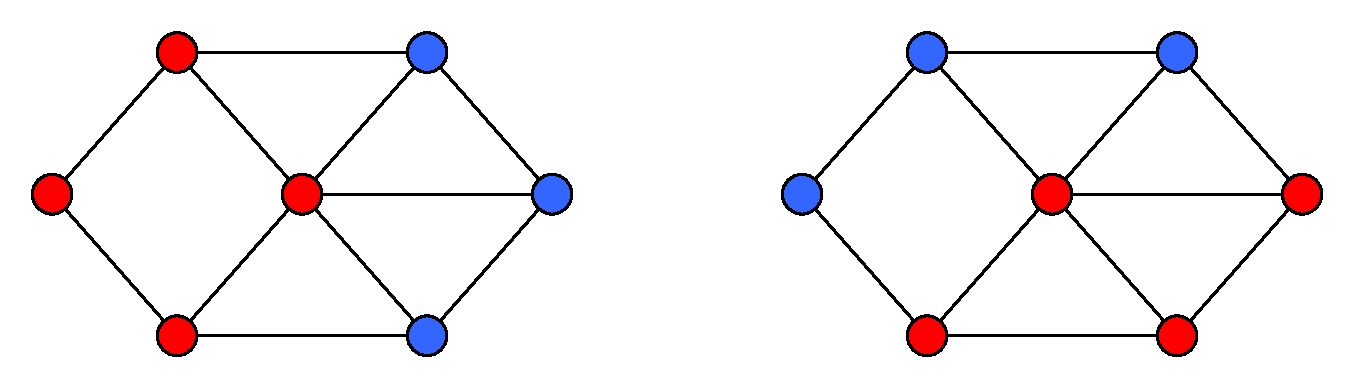
\includegraphics[scale=0.35]{chapter2/fig/badpartition.pdf}
	\caption{Example of bad partition of two equal graphs into two subgraphs} \label{fig:badpartition}
\end{figure}


To cope with this problem, we present an \emph{iterative approach}, where the subgraphs of the initial graphs are allowed to exchange nodes based on the solution $m$ after each iteration of two-level graph matching algorithm. Exchanging rules are based on the affine transformations assigned to each matched pair of the subgraphs.

We consider two matched subgraphs $G^I_k=(V^I_k, E^I_k, D^I_k)$ and  $G^J_p=(V^J_p, E^J_p, D^J_p)$. Based on the matching between the nodes of this pair we apply \emph{RANSAC}~\cite{RANSAC} to estimate two \emph{affine transformations} $T_{kp}:V^I_k\rightarrow V^J_p$ and $T_{pk}:V^J_p\rightarrow V^I_k$. From this two transformations we select the one with smaller transformation error. The transformation error is defined as follows. For each node $v_i\in V^I_k$ we calculate the error between its matched node $m(v_i) = v_j\in V^J_p$ and its projection $T_{kp}(v_i)$: 
\begin{equation} \label{eq:err_v}
err(v_i) = \|T_kp(v_i) - m(v_i)\|_{l_2}
\end{equation}
The error of the estimated affine transformation $T_{kp}$ (analog for  $err(T_{pk})$) is then defined as
\begin{equation} \label{eq:err_T}
err(T_{kp}) = \median_{v_i\in V^I_k}err(v_i)
\end{equation}

For the transformation with the smallest error we calculate its inverse transformation and associate both of them with the subgraph match $(a_k, a_p)$. For simplicity we preserve the notation $T_{kp}$ and $T_{pk}$ for the transformations related to the subgraph match $(a_k, a_p)$.

In this way we can associate to each subgraph pair with more than $3$ node correspondences \footnote{we need at least $3$ pair of correspondences to be able to estimate an affine transformation} the estimated affine transformation of their nodes.

\textit{Rule $1$}

If the transformation describes well the matching between the subgraphs nodes (i.e.\ the transformation error~\ref{eq:err_T} is small), then we include nodes near $T_{kp}(V^I)$, $T_{pk}(V^J)$ in corresponding subgraph with the confidence value equal to $e^{-\min(err(T_{kp}), err(T_{pk}))}$. If one node was selected by several subgraphs, it will be included in the subgraph with the biggest associated confidence value.

\textit{Rule $2$}

If there are subgraph with less then $3$ nodes, we shift this nodes to the subgraphs of their nearest neighbors. For this nodes $err(v)=M$ (see Eq.~\ref{eq:err_v}), where $M$ is some big constant. 

The described approach for subgraph reorganization is summarized in Algorithm~\ref{alg:update_subgraphs}.

\vspace{20pt}
\begin{algorithm}[H]
	\KwIn{ correspondence matrices between nodes of the initial\\
		   \hspace{45pt}graphs and anchors: $U^{Ia}$, $U^{Ja}$\\
		   \hspace{45pt}list of matches between the subgraphs: $m^a = \{(a_k, a_p)\}$;\\
   		   \hspace{45pt}list of estimated affine transformations for each matched \\
   		   \hspace{45pt}pair: $\{(T_{kp}, T_{pk})\}$ }
	\KwOut{new correspondence matrices $\hat{U}^{Ia}$, $\hat{U}^{Ja}$}
	\nl define subgraphs of the initial graphs based on the correspondence \\
	matrices $U^{Ia}$, $U^{Ja}$: $\{G^I_k\}$ and  $\{G^J_p\}$ \\
	\nl $\hat{U}^{Ia} = \frac{1}{2}U^{Ia}$, $\hat{U}^{Ja} = \frac{1}{2}U^{Ja}$ \\
	\nl \ForEach{matched subgraph pair $(a_k, a_p)$}
			{\eIf{$\left|V^I_k\right|\ge 3$ \textbf{AND} $\left|V^J_p\right|\ge 3$}
				{ 
			      $err = \min(err(T_{kp}), err(T_{pk}))$ \tcp*{ see equations \ref{eq:err_v}, \ref{eq:err_T}}
 			      \If{
 			      	 $\left| err\right| < \epsilon $}   %\tcp*{ matching is reliable}
			         {
%			          \tcc{ confidence of the included node to belong to considering subgraphs equals $\exp(-err)$ }
			          $\hat{U}^{Ja}(v, a_p) = \exp(-err)$ for $v\in T_{kp}(V^{I}_k)$ \\
   		 	          $\hat{U}^{Ia}(v, a_k) = \exp(-err)$ for $v\in T_{pk}(V^{J}_p)$ \\
   		 	         }
   		 	    }
    		 	{shift nodes of too small subgraphs into subgraphs, their nearest neighbors belong to} 
		    }			
	\nl  set in each row of  $\hat{U}^{Ia}$($\hat{U}^{Ja}$) the maximum element to $1$ and all other to $0$\\
	\Return $\hat{U}^{Ia}$, $\hat{U}^{Ja}$
	
	\caption{UpdateSubgraphs}    \label{alg:update_subgraphs}
\end{algorithm}

\FloatBarrier

\subsubsection{Simulated Annealing \textbf{SM}}

After some experiments we found out, that the iterative aproach based on the two-level graph matching and the Algorithm~\ref{alg:update_subgraphs} can stay trapped in local optima.
To cope with this we use additionally ideas of the \emph{Simulated Annealing}.

We consider each of the two graphs separately. In each iteration \emph{after application of the Algorithm~\ref{alg:update_subgraphs}} we randomly try to shift a node to one of its three nearest anchors. The energy state of the system is defined as $E = \sum_{v\in V}err(v)$ (see Eq.~\ref{eq:err_v}). After one node was shifted, the new energy state $E^{new}$ is calculated. Wenn $E^{new}<E$ the shifted node stays in its new subgraph. Otherwise, the move is accepted with the probability $exp(-\frac{E^{new}-E}{T})$, where $T = 1/{it}$ is the current temperature of the system and depends on the iteration number $it$. 

\emph{Afterwards} we apply again the Algorithm~\ref{alg:update_subgraphs}. 

